\documentclass[aspectratio=169]{beamer}

\usepackage{tikz}
\usepackage{amssymb}   % \checkmark in verdict badges and tables
\usepackage{colortbl}  % \cellcolor for green/yellow/red cells
\usepackage{booktabs}  % \toprule/\midrule/\bottomrule
\setbeamertemplate{part page}[default]  % metropolis ships no \partpage template

\setbeamerfont{frametitle}{size=\large}
\setbeamerfont{normal text}{size=\small}

% --- Math in Metropolis: use a serif font for math symbols ---
\usefonttheme[onlymath]{serif}

% --- Custom macros (same style as the seminar deck) ---
\newcommand{\deflab}[2]{%
  \textbf{#1}\par\vspace{0.05cm}%
  {\color{blue!55!black}\itshape #2}\par\vspace{0.05cm}}

\newcommand{\keylab}[1]{\textbf{\color{blue!55!black}#1}}

\newcommand{\verdict}[3]{%
  \hfill\colorbox{#2}{\color{#1}\footnotesize\textbf{#3}}%
  \par\vspace{-0.35cm}}

\newcommand{\sketchbox}[2]{%
  \begin{center}\fbox{%
    \begin{minipage}[c][#1][c]{0.85\linewidth}\centering
      \textit{[live demo / screenshot placeholder]}\\[0.2em]
      \footnotesize #2
    \end{minipage}}\end{center}}

% Monospace helper for flags and file names
\newcommand{\flag}[1]{\texttt{\small #1}}

\usetheme{metropolis}
\usecolortheme{default}
\metroset{block=fill}
\metroset{numbering=fraction}

\usepackage[utf8]{inputenc}
\usepackage[T1]{fontenc}
\usepackage{graphicx}
\usepackage{hyperref}
\usetikzlibrary{arrows.meta, positioning, shapes.misc}

\title{Rotor in Rust}
\subtitle{BTOR2 Models for RISC-V, Symbolic Console Arguments,
          and Interactive Visualization}

\author[J. Begi\'{c} \and D. Wassie]
{Jasmin Begi\'{c} \and Daniel Wassie
 \quad{\small (supervised by Prof.\ Christoph Kirsch)}}

\institute[]
{Paris-Lodron University Salzburg --- Advanced Systems Engineering}
\date{June 24th 2026}

\begin{document}

% =========================================================
% TITLE
% =========================================================
\begin{frame}
  \titlepage
\end{frame}

% =========================================================
% SLIDE — OVERVIEW OF THE TALK
% =========================================================
\begin{frame}{Presentation Overview: One Pipeline, Three Contributions}
  \begin{itemize}\setlength\itemsep{0.4em}
    \item \textbf{Part 1 (\textit{Rotor in Rust})}\\
          \emph{The translator.} Rebuilding a 14\,000-line C tool as a
          modular Rust program --- and why it became $\sim$2\,000$\times$
          faster without doing less work.
    \item \textbf{Part 2 (\textit{Symbolic console arguments})}\\
          \emph{The new capability.} Letting the model checker search over
          everything a user could type on the command line --- the paper's
          own ``future work'', implemented.
    \item \textbf{Part 3 (\textit{Witness visualizer})}\\
          \emph{The human side.} Turning the solver's unreadable answer
          into a step-by-step replay in the browser.
  \end{itemize}
  \vspace{0.15cm}
  \begin{center}
  \small\itshape
  And throughout: how we \textbf{verified} that the new tool can be
  trusted --- benchmark by benchmark, against the original.
  \end{center}
\end{frame}

% =========================
% PART 1: THE PROBLEM & BACKGROUND
% =========================
\part{The Problem and the Pipeline}
\begin{frame}
  \partpage
\end{frame}

% ---------------------------------------------------------
\begin{frame}{The Problem: Testing Can Only Try \emph{Some} Inputs}
  \deflab{Testing}{run the program on chosen inputs; observe behaviour}
  \begin{itemize}\setlength\itemsep{0.2em}
    \item 8 bytes of input $= 2^{64}$ possibilities --- if the one
          crashing input is not among those tried, testing says
          nothing about it.
  \end{itemize}
  \vspace{0.1cm}
  \deflab{Verification (bounded model checking)}{reason about \emph{all}
          inputs at once, up to a bound on execution length}
  \begin{itemize}\setlength\itemsep{0.2em}
    \item The unknown input is treated as algebra --- like solving
          $x + 3 = 7$ without trying every $x$.
    \item Answer is two-sided: either a concrete input that reaches the
          bug, or a \emph{guarantee} that none exists within $k$ steps.
  \end{itemize}
\end{frame}

% ---------------------------------------------------------
\begin{frame}{The Pipeline: From C Program to Verified Answer}
  \begin{center}
  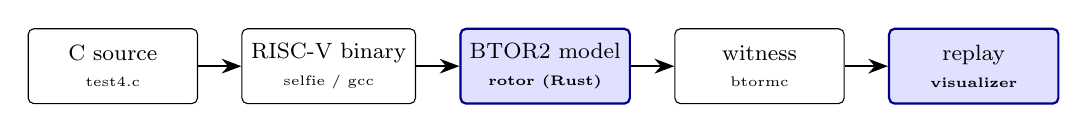
\begin{tikzpicture}[
      box/.style={draw, rounded corners=2pt, minimum height=0.95cm,
                  minimum width=2.15cm, align=center, font=\footnotesize},
      ours/.style={box, fill=blue!12, draw=blue!55!black, thick},
      arr/.style={-{Stealth[length=2.5mm]}, thick}]
    \node[box]                    (src) {C source\\\tiny test4.c};
    \node[box, right=0.55cm of src]  (bin) {RISC-V binary\\\tiny selfie / gcc};
    \node[ours, right=0.55cm of bin] (mod) {BTOR2 model\\\tiny\textbf{rotor (Rust)}};
    \node[box, right=0.55cm of mod]  (sol) {witness\\\tiny btormc};
    \node[ours, right=0.55cm of sol] (vis) {replay\\\tiny\textbf{visualizer}};
    \draw[arr] (src) -- (bin);
    \draw[arr] (bin) -- (mod);
    \draw[arr] (mod) -- (sol);
    \draw[arr] (sol) -- (vis);
  \end{tikzpicture}
  \end{center}
  \vspace{0.1cm}
  \begin{itemize}\setlength\itemsep{0.4em}
    \item Rotor works on the \keylab{compiled binary} --- what is
          verified is what actually runs. \keylab{BTOR2} is the model
          format; \keylab{btormc} the bounded model checker.
    \item Highlighted stages are this project; selfie and btormc are
          unchanged third-party tools.
  \end{itemize}
\end{frame}

% ---------------------------------------------------------
\begin{frame}{What a Rotor Model Contains}
  A machine model is a board game description: \keylab{state},
  \keylab{rules}, and \keylab{forbidden positions}.
  \vspace{0.05cm}
  \begin{columns}[T]
    \column{0.48\linewidth}
      \textbf{State} (one instant of the machine)
      \begin{itemize}\setlength\itemsep{0.2em}
        \item program counter, 32 registers
        \item memory: code, data, heap, stack
        \item kernel: program break, file descriptor, input counters
      \end{itemize}
    \column{0.48\linewidth}
      \textbf{Rules + properties}
      \begin{itemize}\setlength\itemsep{0.2em}
        \item one transition function per state variable ---
              the semantics of every instruction
        \item \textbf{24 bad-state properties}: division by zero,
              segmentation faults, illegal instructions, unknown
              syscalls, target exit code, \dots
      \end{itemize}
  \end{columns}
  \vspace{0.15cm}
  \begin{block}{The solver's single question}
    Starting from the initial state and following the rules, can the
    machine reach a bad state within $k$ steps --- \emph{for any} input?
  \end{block}
\end{frame}

% =========================
% PART 2: ROTOR IN RUST
% =========================
\part{Rotor in Rust}
\begin{frame}
  \partpage
\end{frame}

% ---------------------------------------------------------
\begin{frame}{Why Rebuild Rotor?}
  \begin{columns}[T]
    \column{0.48\linewidth}
      \textbf{The original (rotor.c)}
      \begin{itemize}\setlength\itemsep{0.3em}
        \item one file, $\sim$14\,000 lines of C*
        \item hundreds of file-level globals
        \item per-core state in parallel arrays
        \item hard to read, extend, integrate
      \end{itemize}
    \column{0.48\linewidth}
      \textbf{The rewrite (Rust)}
      \begin{itemize}\setlength\itemsep{0.3em}
        \item modular crate, one file per concern:
              builder, machine, decoder, properties
        \item typed node graph (\texttt{enum Op}) instead of
              15-slot heap arrays
        \item explicit four-phase pipeline, no globals
      \end{itemize}
  \end{columns}
  \vspace{0.15cm}
  \begin{block}{Same job, same checks}
    The rewrite emits the \textbf{same 24 bad-state properties} ---
    same names, same order, same predicates, re-derived line by line
    from \texttt{rotor.c}.
  \end{block}
\end{frame}

% ---------------------------------------------------------
\begin{frame}{The Duplicate-Check Story (Where the Speed Comes From)}
  Both rotors reuse syntactically identical subexpressions to keep
  models small. The difference is \emph{how they look for duplicates}:
  \vspace{0.2cm}
  \begin{columns}[T]
    \column{0.48\linewidth}
      \deflab{C rotor}{linear scan}
      \begin{itemize}\setlength\itemsep{0.25em}
        \item every new node: walk the list of \emph{all} previous nodes
        \item $\mathcal{O}(N)$ per node $\Rightarrow$
              $\mathcal{O}(N^2)$ total
        \item had to be \emph{disabled} for binary loading to stay usable
      \end{itemize}
    \column{0.48\linewidth}
      \deflab{Rust rotor}{hash map}
      \begin{itemize}\setlength\itemsep{0.25em}
        \item every new node: one $\mathcal{O}(1)$ lookup keyed by
              (operator, sort, operands)
        \item $\mathcal{O}(N)$ total
        \item stays \emph{on everywhere}, including binary loading
      \end{itemize}
  \end{columns}
  \vspace{0.15cm}
  {\footnotesize At $N \approx 110$k nodes: $\sim$6 billion comparisons
  vs.\ $\sim$110k lookups --- the check itself is identical.}
\end{frame}

% ---------------------------------------------------------
\begin{frame}{The Selfie Challenge: ``Just Model All of Selfie''}
  Input: selfie self-compiled to RISC-U --- \textbf{43\,406
  instructions}, the largest natural benchmark.
  \vspace{0.1cm}
  \begin{center}
  \begin{tabular}{lrrr}
    \toprule
    Metric & C rotor & Rust rotor & ratio\\
    \midrule
    model generation time & 106\,s & \textbf{47\,ms} &
      $\sim$2\,250$\times$\\
    peak memory           & 431\,MB & \textbf{20\,MB} &
      $\sim$21$\times$\\
    output size           & 10.6\,MB & \textbf{3.1\,MB} &
      3.4$\times$\\
    validated by btormc   & --- & \checkmark & \\
    \bottomrule
  \end{tabular}
  \end{center}
  \vspace{0.1cm}
  \begin{itemize}\setlength\itemsep{0.2em}
    \item \textbf{Not} from doing less: same 24 properties, and the
          models behave identically under btormc (Part 4).
          Consistent with $\mathcal{O}(N^2)$ vs.\ $\mathcal{O}(N)$.
  \end{itemize}
\end{frame}

% ---------------------------------------------------------
\begin{frame}{``Disable It and See If the Universe Ends''}
  The supervisor's experiment: turn the duplicate check \emph{off} in
  both tools and compare.
  \vspace{0.1cm}
  \begin{columns}[T]
    \column{0.48\linewidth}
      \deflab{C rotor, \texttt{reuse\_lines = 0}}{the universe ends}
      \begin{itemize}\setlength\itemsep{0.25em}
        \item crashes 0.08\,s in:\\
              {\footnotesize\texttt{ite then sort mismatch error}}
        \item the C generator \emph{relies} on reuse for node identity
              --- the check is load-bearing, not just an optimization
      \end{itemize}
    \column{0.48\linewidth}
      \deflab{Rust rotor, \flag{--no-cse}}{the universe survives}
      \begin{itemize}\setlength\itemsep{0.25em}
        \item models grow $\sim$1.43$\times$\\
              {\footnotesize (selfie: 110\,904 $\to$ 159\,018 lines)}
        \item still valid BTOR2, same solver verdicts
        \item dedup is \emph{semantically neutral} by construction
      \end{itemize}
  \end{columns}
  \vspace{0.12cm}
  \begin{block}{Take-away}
    The speed difference is the \emph{data structure}, not a difference
    in what gets deduplicated.
  \end{block}
\end{frame}

% ---------------------------------------------------------
\begin{frame}{Making the Machine Faithful (What ``Correct'' Required)}
  Same properties were not enough --- the modeled \emph{machine}
  had to be identical:
  \begin{itemize}\setlength\itemsep{0.3em}
    \item \keylab{Memory \& registers start zeroed} --- else the
          solver invents memory contents (false counterexamples).
    \item \keylab{Exact segment geometry} --- page-aligned heap,
          stack at $[\texttt{0xFFFFF800},\,2^{32})$, program break
          at heap start.
    \item \keylab{Boot image} --- concrete argc/argv stack layout at
          start-up, exactly like selfie's boot loader.
    \item \keylab{Read syscall semantics} --- one input byte per
          transition, PC stalled while reading; exit stalls forever.
    \item \keylab{All 24 properties} in the C output's exact emission
          order, so btormc property indices line up.
  \end{itemize}
\end{frame}

% =========================
% PART 3: SYMBOLIC ARGV
% =========================
\part{Symbolic Console Arguments}
\begin{frame}
  \partpage
\end{frame}

% ---------------------------------------------------------
\begin{frame}{The Gap: A Whole Class of Bugs Was Invisible}
  \begin{itemize}\setlength\itemsep{0.4em}
    \item Original rotor: the solver explores inputs read from
          \keylab{stdin} only.
    \item Command-line arguments were \keylab{fixed} in the model ---
          always an empty command line.
    \item Consequence: any bug that fires only for a specific argument
          is \emph{structurally unreachable}. The solver was never
          allowed to look.
  \end{itemize}
  \vspace{0.25cm}
  \begin{block}{From the rotor paper (\S 3 and Conclusions)}
    \itshape ``the stack segment is initialized with console arguments
    of executables. However, support of console arguments as symbolic
    input is future work.''
  \end{block}
  \vspace{0.1cm}
  \centering\small That future-work item --- by name --- is what Part 2
  implements.
\end{frame}

% ---------------------------------------------------------
\begin{frame}{What ``Symbolic'' Means Here}
  \deflab{Symbolic value}{left open for the solver to choose, instead of
          fixed to one concrete value}
  \begin{itemize}\setlength\itemsep{0.3em}
    \item At process start the OS writes argument characters into stack
          memory as ordinary bytes (plus count and pointers).
    \item \flag{--symbolic-argv} builds the \emph{same layout}, but
          \texttt{argv[1..N]} content bytes become
          \keylab{uninitialized 8-bit states} (no \texttt{init}).
    \item Think Sudoku: most cells pre-filled; the blanks are the
          argument characters; the solver fills them
          \emph{looking for a bad state}.
  \end{itemize}
  \vspace{0.1cm}
  \begin{block}{Why this mechanism is the right one}
    The paper's Definition 1 formalizes machine input as
    \emph{uninitialized states} --- symbolic argv uses exactly that
    device, fitting the existing soundness framework.
  \end{block}
\end{frame}

% ---------------------------------------------------------
\begin{frame}{The Stack Layout at Boot (Symbolic Mode)}
  \begin{center}
  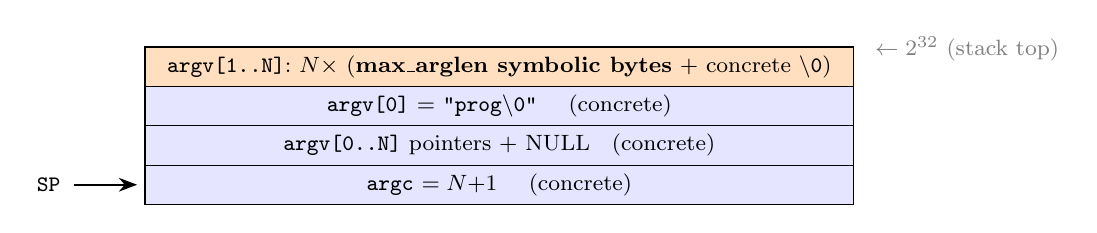
\begin{tikzpicture}[yscale=0.5, font=\footnotesize]
    % string area
    \fill[orange!25] (0,6) rectangle (9,7);
    \draw (0,6) rectangle (9,7);
    \node at (4.5,6.5) {\texttt{argv[1..N]}: $N \times$
      (\textbf{max\_arglen symbolic bytes} + concrete \texttt{\textbackslash0})};
    \fill[blue!10] (0,5) rectangle (9,6);
    \draw (0,5) rectangle (9,6);
    \node at (4.5,5.5) {\texttt{argv[0]} = \texttt{"prog\textbackslash0"}
      \hspace{1em}(concrete)};
    \fill[blue!10] (0,4) rectangle (9,5);
    \draw (0,4) rectangle (9,5);
    \node at (4.5,4.5) {\texttt{argv[0..N]} pointers + NULL
      \hspace{0.6em}(concrete)};
    \fill[blue!10] (0,3) rectangle (9,4);
    \draw (0,3) rectangle (9,4);
    \node at (4.5,3.5) {\texttt{argc} $= N{+}1$ \hspace{1em}(concrete)};
    \draw[-{Stealth}, thick] (-0.9,3.5) -- (-0.1,3.5);
    \node[anchor=east] at (-0.95,3.5) {\texttt{SP}};
    \node[anchor=west, gray] at (9.15,6.95) {$\leftarrow 2^{32}$ (stack top)};
  \end{tikzpicture}
  \end{center}
  \begin{itemize}\setlength\itemsep{0.15em}
    \item Only the \colorbox{orange!25}{highlighted} bytes are open;
          everything else is concrete.
    \item Arguments are read through \emph{ordinary loads} --- decoder,
          memory system, and properties untouched.
  \end{itemize}
\end{frame}

% ---------------------------------------------------------
\begin{frame}{Design Choices (and Their Honest Trade-offs)}
  \begin{itemize}\setlength\itemsep{0.35em}
    \item \keylab{argc is fixed at generation time}
          (\flag{--num-symbolic-args~N}). The solver explores argument
          \emph{content}, not count --- symbolic argc would need a
          dynamic stack layout.
    \item \keylab{Bounded length} (\flag{--max-arglen~K}) --- same
          philosophy as the paper's bounded input buffer
          (``size of model input is bounded'').
    \item \keylab{Fixed-slot strings.} Real \texttt{execve} packs
          strings end-to-end; we use fixed slots. Identical behaviour
          for programs that treat arguments as C strings (all of ours);
          a caveat only for out-of-bounds pointer walkers.
    \item \keylab{Interior zero bytes allowed} --- corresponds to a
          shorter real-world string.
  \end{itemize}
  {\footnotesize Where the paper is silent, we chose --- and all
  choices keep the model finite and static.}
\end{frame}

% ---------------------------------------------------------
\begin{frame}{Validation: Five Programs Whose Bugs Live Only in argv}
  All five are C* programs; none reads stdin --- so \emph{none} of
  these bugs is reachable with stdin-only symbolic input.
  \vspace{0.15cm}
  \begin{center}
  \footnotesize
  \begin{tabular}{lll}
    \toprule
    Test & Bug fires when\dots & Solver must find\\
    \midrule
    test1 & \texttt{argv[1][0] == 67} (\texttt{'C'}) & one exact byte\\
    test2 & $\texttt{argv[1][0]}{\cdot}256 + \texttt{argv[1][1]} = 16706$
          & two bytes, ordered\\
    test3 & \texttt{argv[1][0]} $\neq 0$ \textbf{and}
            \texttt{argv[1][1]} $= 0$ & a length property\\
    test4 & \texttt{argv[1][0]='X'} \textbf{and}
            \texttt{argv[2][0]='Y'} & two \emph{arguments} at once\\
    test5 & \texttt{argv[1][0]} + \texttt{argv[1][1]} $= 200$
          & arithmetic relation\\
    \bottomrule
  \end{tabular}
  \end{center}
  \vspace{0.2cm}
  \begin{block}{Verified result (test1)}
    \texttt{bad-exit-code} SATISFIABLE at $k = 67$; witness
    \texttt{argv[1][0]} $= \texttt{0x43} = $ \texttt{'C'} --- found
    through three pointer dereferences. All five solve in seconds.
  \end{block}
\end{frame}

% =========================
% PART 4: VISUALIZER
% =========================
\part{The Witness Visualizer}
\begin{frame}
  \partpage
\end{frame}

% ---------------------------------------------------------
\begin{frame}[fragile]{The Problem: The Answer Is Unreadable}
  What btormc actually returns when it finds a bug:
  \begin{example}{}
\begin{verbatim}
sat
b23
#0
3 01000011 argv[1][0]#0
4 10000010 argv[1][1]#0
1 [...0001101] 00000000 initial-data-base@0
...thousands of lines keyed to internal node numbers...
\end{verbatim}
  \end{example}
  \vspace{0.15cm}
  \begin{itemize}\setlength\itemsep{0.3em}
    \item Sound, complete --- and unreadable. A result that cannot be
          \emph{read} persuades no one.
  \end{itemize}
\end{frame}

% ---------------------------------------------------------
\begin{frame}{The Visualizer: the Model as a Living Graph}
  Browser app, no installation --- also hosted online.
  \begin{columns}[T]
    \column{0.52\linewidth}
      \textbf{Model view}
      \begin{itemize}\setlength\itemsep{0.25em}
        \item every machine part is a node; shape/colour by category
              (red octagons = bad states, green = state, \dots)
        \item cone-of-influence and depth-limited views,
              collapse/expand, clumping, search, PNG/SVG export
      \end{itemize}
    \column{0.44\linewidth}
      \textbf{Witness replay}
      \begin{itemize}\setlength\itemsep{0.25em}
        \item load model + witness, press play
        \item per-step inspector: changed values, chosen input bytes,
              fired bad state
        \item timeline scrubber, keyboard shortcuts, drag \& drop
      \end{itemize}
  \end{columns}
  \vspace{0.2cm}
  \begin{itemize}\setlength\itemsep{0.25em}
    \item 12 built-in examples, including all five argv tests with
          their solved witnesses.
    \item Live: {\small\url{https://jaspek.github.io/rotor-rust/}}
  \end{itemize}
\end{frame}

% ---------------------------------------------------------
\begin{frame}{Demo}
  \sketchbox{5.2cm}{Live demo: load \texttt{argv test4} from the
    example picker --- watch the solver's chosen bytes
    (\texttt{argv[1][0]='X'}, \texttt{argv[2][0]='Y'}) drive the
    program to the bad exit, step by step.}
\end{frame}

% =========================
% PART 5: TRUST & EQUIVALENCE
% =========================
\part{Can the New Tool Be Trusted?}
\begin{frame}
  \partpage
\end{frame}

% ---------------------------------------------------------
\begin{frame}{The Standard of Evidence}
  \begin{block}{Supervisor's feedback (verbatim)}
    \itshape ``There is no way to know that [the models are
    equivalent] \dots\ So basically check them yourself.''
  \end{block}
  \vspace{0.2cm}
  \begin{itemize}\setlength\itemsep{0.45em}
    \item Full formal equivalence of two model generators is
          undecidable --- the paper itself lists formal verification of
          rotor as future work.
    \item Our checkable criterion: for the same binary, btormc must
          report the \keylab{same bad-state property} (same index!) at
          the \keylab{same least bound $k$} from both rotors' models.
    \item An independent referee: if the models differed anywhere the
          program's execution touches, the property or the step count
          would differ.
  \end{itemize}
\end{frame}

% ---------------------------------------------------------
\begin{frame}{Finding Real Bugs in Our Own Tool (the Honest Part)}
  The deep check caught us three times before it confirmed us:
  \vspace{0.15cm}
  \begin{itemize}\setlength\itemsep{0.45em}
    \item \keylab{Unconstrained memory.} Segments and registers had no
          init $\Rightarrow$ solver-invented contents $\Rightarrow$
          spurious counterexamples. \emph{Fix: zero everything, like
          the reference.}
    \item \keylab{Wrong geometry.} 2\,GB address space, unaligned heap,
          program break at the wrong address. \emph{Fix: exact C
          constants, verified byte-for-byte.}
    \item \keylab{Read syscall did not deliver bytes.} The input buffer
          existed but was never read --- programs branched on garbage.
          \emph{Fix: full port --- one byte per transition, PC stall,
          exact return values.}
  \end{itemize}
  \vspace{0.15cm}
  {\footnotesize Each fix: rebuild $\to$ regenerate $\to$ catbtor +
  btormc validation $\to$ deep re-run. Only then the next step.}
\end{frame}

% ---------------------------------------------------------
\begin{frame}{Results: Same Property, Same Step --- Benchmark by Benchmark}
  %% TODO before the talk: fill in the remaining rows from
  %% benchmarks/deep_equivalence_results.csv when the harness completes.
  \begin{center}
  \footnotesize
  \begin{tabular}{lllc}
    \toprule
    Benchmark & C rotor & Rust rotor & match\\
    \midrule
    division-by-zero & division-by-zero @ 76 & division-by-zero @ 76 &
      \cellcolor{green!20}\checkmark\\
    invalid-memory-access & store-invalid-addr @ 79 &
      store-invalid-addr @ 79 & \cellcolor{green!20}\checkmark\\
    memory-access-fail & load-seg-fault @ 66 & load-seg-fault @ 66 &
      \cellcolor{green!20}\checkmark\\
    nested-if-else & bad-exit-code @ 100 & bad-exit-code @ 100 &
      \cellcolor{green!20}\checkmark\\
    nested-if-else-rev & bad-exit-code @ 103 & bad-exit-code @ 103 &
      \cellcolor{green!20}\checkmark\\
    nested-recursion-fail & UNSAT @ 1500 & UNSAT @ 1500 &
      \cellcolor{green!20}\checkmark\\
    recursive-ackermann & bad-exit-code @ 152 & bad-exit-code @ 152 &
      \cellcolor{green!20}\checkmark\\
    recursive-factorial & bad-exit-code @ 119 & bad-exit-code @ 119 &
      \cellcolor{green!20}\checkmark\\
    recursive-fibonacci & bad-exit-code @ 118 & bad-exit-code @ 118 &
      \cellcolor{green!20}\checkmark\\
    \bottomrule
  \end{tabular}
  \end{center}
  \vspace{0.1cm}
  {\footnotesize Five property types; recursion matched step-exactly.
  Reproducible: \texttt{run\_deep\_equivalence.ps1}, kmax = 1500.}
\end{frame}

% =========================
% CONCLUSIONS
% =========================
\part{Conclusions}
\begin{frame}
  \partpage
\end{frame}

% ---------------------------------------------------------
\begin{frame}{What We Delivered}
  \begin{itemize}\setlength\itemsep{0.55em}
    \item \keylab{Rotor in Rust} --- modular, $\sim$2\,250$\times$
          faster model generation, 21$\times$ less memory, same 24
          checks; behavioural equivalence verified per benchmark by an
          independent solver.
    \item \keylab{Symbolic console arguments} --- the paper's named
          future-work item, implemented with the paper's own formal
          device (uninitialized states); five argv-only bugs found
          within seconds, none reachable via stdin.
    \item \keylab{Witness visualizer} --- the solver's answer as an
          interactive, step-by-step replay; live online with 12
          examples.
  \end{itemize}
  \vspace{0.1cm}
  \begin{block}{One sentence}
    From a compiled binary to a \emph{readable} verified answer ---
    end to end, faster, and with a wider input space than before.
  \end{block}
\end{frame}

% ---------------------------------------------------------
\begin{frame}{Future Work}
  \begin{itemize}\setlength\itemsep{0.5em}
    \item \textbf{Symbolic argc / packed string layouts} --- explore
          argument \emph{count} symbolically; model the exact
          \texttt{execve} memory packing.
    \item \textbf{More symbolic surfaces} --- environment variables,
          file contents (requires file-descriptor modelling).
    \item \textbf{Complete the equivalence matrix} --- all 18
          benchmarks plus selfie's self-model at depth; add 2--3 deep
          checks to CI.
    \item \textbf{Smarter deduplication} --- semantic equivalences
          (commutativity, identities) beyond the syntactic check.
    \item \textbf{Visualizer} --- diffing two witnesses; live solver
          integration.
  \end{itemize}
\end{frame}

% ---------------------------------------------------------
\begin{frame}
  \centering
  \Huge{\textbf{Thank You for your Attention}}
  \vspace{0.8cm}

  \normalsize
  \url{https://github.com/jaspek/rotor-rust}\\
  \url{https://jaspek.github.io/rotor-rust/}
\end{frame}

% =========================================================
% REFERENCES
% =========================================================
\begin{frame}[allowframebreaks]{Selected References}
  \footnotesize
  \begin{itemize}\setlength\itemsep{0.4em}
    \item \textbf{Bolotina, A., Kirsch, C.\ M., Muroya Lei, S.,
          Pleschinger, M.\ \& Shorabi, A.} Rotor: Generating RISC-V
          machine models for bounded model checkers and SMT solvers.
          \textit{(the rotor paper; basis of this project)}
    \item \textbf{Bolotina, A.\ et al.} Bitme: Incremental concurrent
          bounded model checking of RISC-V machine models using binary
          decision diagrams. \textit{Submitted to CAV 2026.}
    \item \textbf{Niemetz, A., Preiner, M., Wolf, C.\ \& Biere, A.\
          (2018).} BTOR2, BtorMC and Boolector 3.0.
          \textit{Proc.\ CAV}, 587--595.
    \item \textbf{Biere, A., Cimatti, A., Clarke, E.\ \& Zhu, Y.\
          (1999).} Symbolic model checking without BDDs.
          \textit{Proc.\ TACAS}, 193--207.
    \item \textbf{Kirsch, C.\ (2017).} Selfie and the basics.
          \textit{Proc.\ ACM Onward!}
    \item \textbf{Cadar, C., Dunbar, D.\ \& Engler, D.\ R.\ (2008).}
          KLEE: Unassisted and automatic generation of high-coverage
          tests for complex systems programs. \textit{Proc.\ OSDI},
          209--224.
    \item \textbf{Waterman, A.\ \& Asanovi\'{c}, K.\ (eds.)\ (2017).}
          The RISC-V instruction set manual, volume I: User-level ISA.
    \item Project repository:
          \url{https://github.com/jaspek/rotor-rust} --- includes
          \texttt{EQUIVALENCE\_PLAN.md}, \texttt{P2\_RESULTS.md}, and
          the reproducible benchmark harness.
  \end{itemize}
\end{frame}

\end{document}
